\def\year{2015}
%File: formatting-instruction.tex
\documentclass[letterpaper]{article}
\usepackage{aaai}
\usepackage{times}
\usepackage{helvet}
\usepackage{courier}
\frenchspacing
\setlength{\pdfpagewidth}{8.5in}
\setlength{\pdfpageheight}{11in}
\pdfinfo{
/Title (Insert Your Title Here)
Matheus Redecker (Put All Your Authors Here, Separated by Commas)}
\setcounter{secnumdepth}{0}  

\usepackage[portuguese]{babel}
\usepackage[utf8]{inputenc}
\usepackage{graphicx,url}

 \begin{document}
 \nocopyright
% The file aaai.sty is the style file for AAAI Press 
% proceedings, working notes, and technical reports.
%
\title{ Aprendizado por Reforço  }
\author{Matheus Redecker, Leonardo Gubert\\
Pontifícia Universidade Católica do Rio Grande do Sul - PUCRS\\
Av. Ipiranga, 6681 \\
Porto Alegre, Rio Grande do Sul\\
}
\maketitle

\section{Introdução}
Neste artigo será apresentada uma alternativa de solução para o labirinto de Hyrule utilizando o algoritmo de aprendizado por reforço chamado Q-learning. Este problema visa gerar uma política para que o agente atinja o objetivo da maneira mais otimizada possível, independente das ações tomadas dado o aspecto estocástico do problema. O mapa é composto por espaços vazios onde o agente pode se mover, espaços preenchidos onde não se pode atravessar, um tesouro que é o estado final do jogo e diamantes (rupees) que podem estar espalhados pelos espaços vazios no mapa. A recompensa por obter o baú é de 50 pontos, pegar um diamante vale 5 pontos e cada ação realizada é descontado 1 ponto. Para cada estado é calculado um valor de utilidade para cada possível ação, assim determina-se qual deve ser a próxima ação a ser tomada. Existe ainda, 30\% de probabilidade da ação tomada resultar em um movimento não esperado que deixe o agente em alguma outra posição adjacente, sendo 15\% para cada lado, o que torna o problema não determinístico e implica no agente poder fazer caminhos diferentes dado o mesmo plano de execução. \\
Nas próximas seções será apresentado o algoritmo utilizado para resolver o problema, os resultados obtidos e por fim uma conclusão onde mostramos as dificuldades de implementação e as experiências adquiridas. 

\section{Q-Learning}
Q-Learning é um algoritmo de aprendizado por reforço que visa achar a política ótima para um MDP (Markovian Decision Process) utilizando uma fórmula para atualizar o aprendizado de cada estado. A fórmula é dada por  $Q(s,a) \leftarrow Q(s,a) + \alpha * (R(s) + \gamma *  max_{a} Q(s',a') - Q(s,a)) $, onde $s$ é um estado, $a$ uma ação, $Q(s,a)$ a utilidade do par estado e ação, e $R(s)$ a recompensa do estado. $\alpha$ é calculado baseado no número de vezes que o estado foi visitado e $\gamma$ é o fator de desconto (ao qual atribuímos a constante $0.9$). Este algoritmo consiste em calcular, a partir de um estado e uma ação, o valor Q, que irá representar a utilidade para o estado anterior dada a ação. Em outras palavras, o algoritmo extrai qual o ganho para o agente do par estado e ação anterior ao estado atual, executados várias vezes para cada estado e propagando o valor do estado terminal para os demais estados.  \\ 
Para aplicar esse algoritmo e resolver o problema foram utilizadas duas estruturas de dado: Uma para guardar a frequência que cada par estado e ação foi visitado e outra para armazenar os valores de utilidade de cada par. O algoritmo utiliza o estado seguinte para calcular a utilidade do anterior, então as informações do estado $a$ e ação anteriores também são armazenadas e subistituidas a cada novo passo no algoritmo. Para cada calculo de utilidade é necessario seguir os seguintes passos. 

\begin{itemize}
\item Pegar a frequência para o par estado e ação.
\item Calcular $\alpha$ que é dado por: \\
        (1/(frequência+1)) * frequência.
\item Incrementar a frequência.
\item Atribuir 0.9 para $\gamma$.
\item Calcular qual a melhor ação para o estado atual.
\item Aplicar a formula para o par (estado, ação) anterior.
\end{itemize}


\section{Experimentos}
Para testar o algoritmo utilizamos um conjunto de quatro mapas fornecido pelo professor, sendo dois deles simples para o entendimento do problema e dois mais complexos. Para exemplificar, pegamos um exemplo de cada categoria e apresentaremos o plano gerado e a sua convergência ao longo dos episódios do treinamento. O problema para validar o algoritmo foi o problema fácil, onde o agente tem que seguir por apenas um caminho para chegar a recompensa, o mapa é de dimensões pequenas e a quantidade de estados baixa, fazendo que o plano gerado seja bem simples para a validação do algoritmo. Uma vez que o plano tenha sido gerado de forma correta, o problema de complexidade media se é apresentado com uma quantidade de estados maior e uma dimensão maior, como o primeiro problema existe um caminho que chega ao objetivo mais rápido que os demais.
A aplicação do algoritmo é feita até que haja convergência em cada estado alcançável do mapa, ou seja, cada estado terá quatro possibilidades de ação iniciais, mas após a execução do algoritmo uma melhor ação é encontrada. Isso é chamado de treino. Cada vez que se obtém uma convergência temos um treino bem sucedido, mas para que isso aconteça é necessário que a diferença da convergência entre 2 treinos esteja dentro de uma margem de erro estipulada. Após uma determinada quantidade de treinos, como podemos ver nas figuras \ref{easy_conv} e \ref{medi_conv} o valor de convergência tende a variar cada vez menos entre treinos, até que tenham a diferença dentro da margem especificada ($<0.1$, para estes problemas)\\

\begin{figure}[ht]
\centering
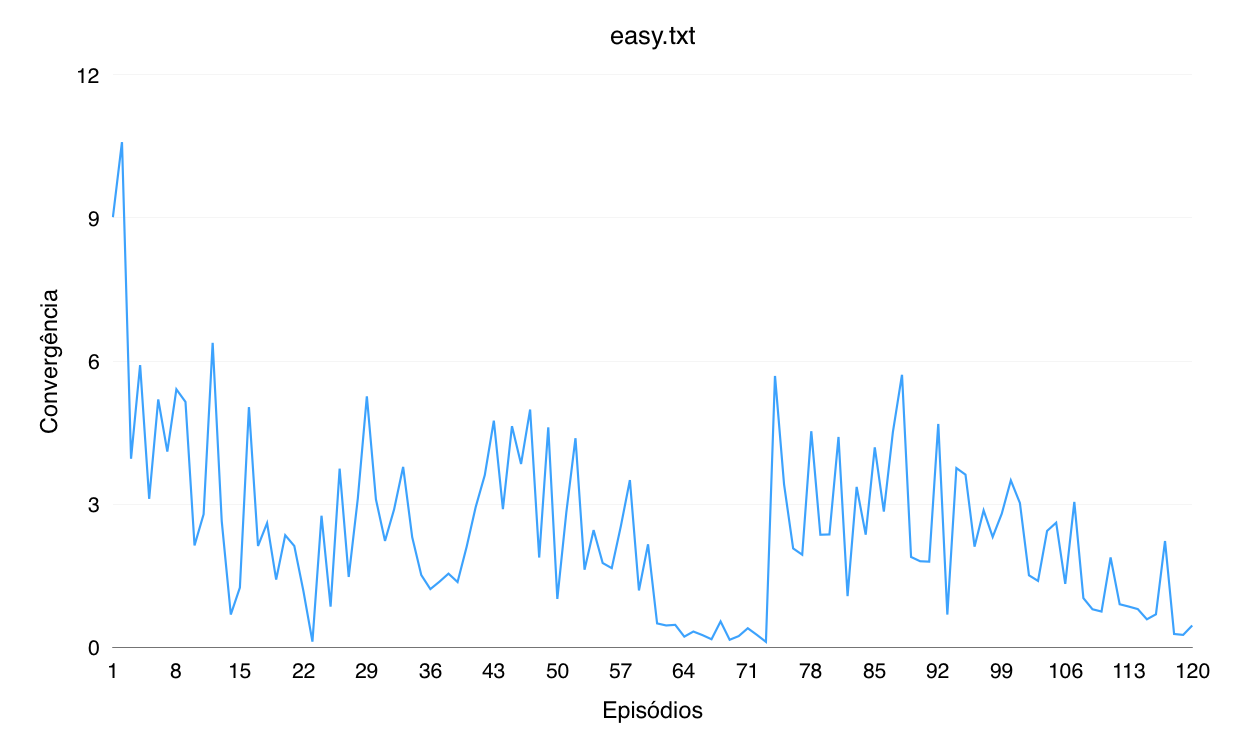
\includegraphics[scale=0.192]{easy_map.png} %192
\caption{}
\label{easy_conv}
\end{figure}

\begin{figure}[ht]
\centering
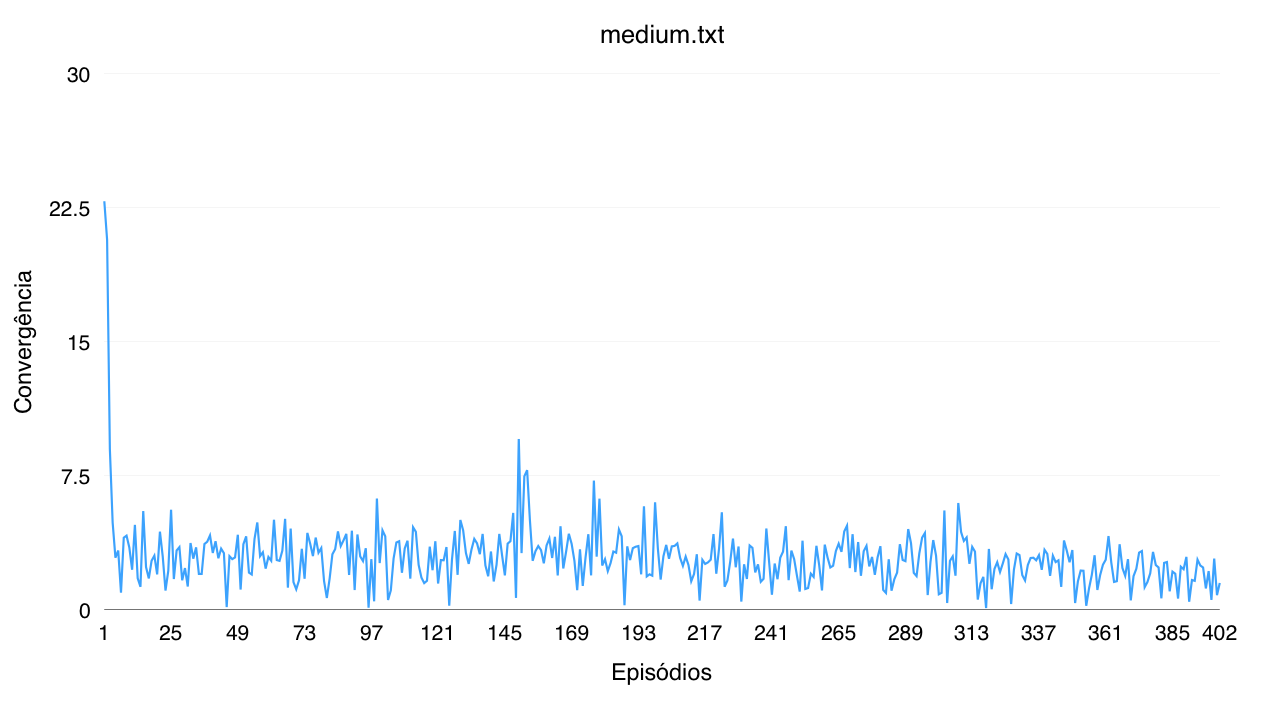
\includegraphics[scale=0.18]{medium_map.png}
\caption{}
\label{medi_conv}
\end{figure}

O plano gerado pode ser visto nas figuras \ref{map_easy} e \ref{map_medium}. Como podemos ver o valor do estado terminal se propaga para os demais estados. Cada estado determina qual a melhor ação (a que leva para mais próximo do baú), que é onde a recompensa está. Quanto mais claro, maior é o valor de utilidade para aquela ação no estado. Como estamos em um ambiente estocástico o agente pode às vezes cair em um estado que desvia do caminho, mas mesmo assim o plano consegue enviá-lo para o estado terminal. Os estados mais escuros representam estados que não contribuem para o objetivo, mas eles contêm um valor muito pequeno apenas para apontar a ação que irá retomar o agente para o caminho correto. Como os diamantes acrescentam 40 na recompensa final, eles não propagam tão fortemente quanto o objetivo, então nos exemplos que continham o diamante apenas os estados em sua adjacencia ficam com cor clara, mas entram em conflito quando há um baú próximo.

\begin{figure}[ht]
\centering
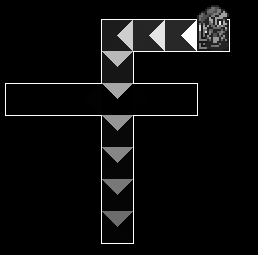
\includegraphics[scale=0.6]{easy.png}
\caption{}
\label{map_easy}
\end{figure}

\begin{figure}[ht]
\centering
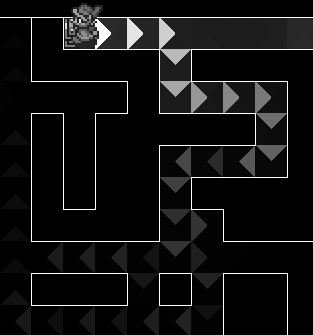
\includegraphics[scale=0.5]{medium.png}
\caption{}
\label{map_medium}
\end{figure}
\newpage{}
\section{Conclusão}

Na realização do trabalho encontramos algumas dificuldades para entender como aplicar a fórmula de atualização da tabela do algoritmo no contexto do jogo, não ficou claro para nós como devíamos usar os estados do agente. Na primeira versão calculamos para todos os estados dado todas as ações possíveis, o que levava a um plano razoável, mas devido a alta complexidade não era possível executar os problemas medianos. Após algum tempo pensando e uma visita a monitoria percebemos que deveríamos utilizar os estados que estão presentes no agente ($s$ e $prev$\_$s$), então utilizamos esses valores fornecidos para aplicar a formula e assim obtivemos uma política razoável para cada um dos problemas. \\
Quando temos mapas que são muito abertos, ou seja, quase não tem espaços preenchidos, temos alguns problemas quanto aos planos gerados, algumas vezes os estados apresentam a melhor ação onde não deveriam, chegamos a conclusão que isso vem do fato da quantidade de cálculos de atualização de utilidade, pois em algum momento os valores não representam a melhor ação para aquele estado. \\
Um problema que encontramos foi ver qual o valor de utilidade para cada par estado e ação, apenas com a indicação de cor ficava complicado analisar se o backpropagation estava propagando o valor correto ou ainda se a tabela estava coerente com o que deveria apresentar. Para resolver esse problema foi implementado um método para mostrar a tabela varrendo todos os estados após a geração do plano.


\end{document}
